\documentclass[tikz,border=2]{standalone}
%% \usepackage{amsfonts}
\usepackage{lmodern} % enhanced version of computer modern
\usepackage[T1]{fontenc} % for hyphenated characters
\usepackage{amssymb}
\usepackage{amsmath}
\usepackage{amsthm}
%
\usetikzlibrary{decorations.pathreplacing,shadows,arrows,shapes,positioning,calc,backgrounds,fit}
\newcommand{\mA}{\mathcal{A}}
\newcommand{\mB}{\mathcal{B}}
\newcommand{\mC}{\mathcal{C}}
\newcommand{\mI}{\mathcal{I}}
\newcommand{\mN}{\mathcal{N}}
\newcommand{\mP}{\mathcal{P}}
\newcommand{\mR}{\mathcal{R}}
\newcommand{\mS}{\mathcal{S}}
\newcommand{\mY}{\mathcal{Y}}
% Define the layers to draw the diagram
%
\begin{document}
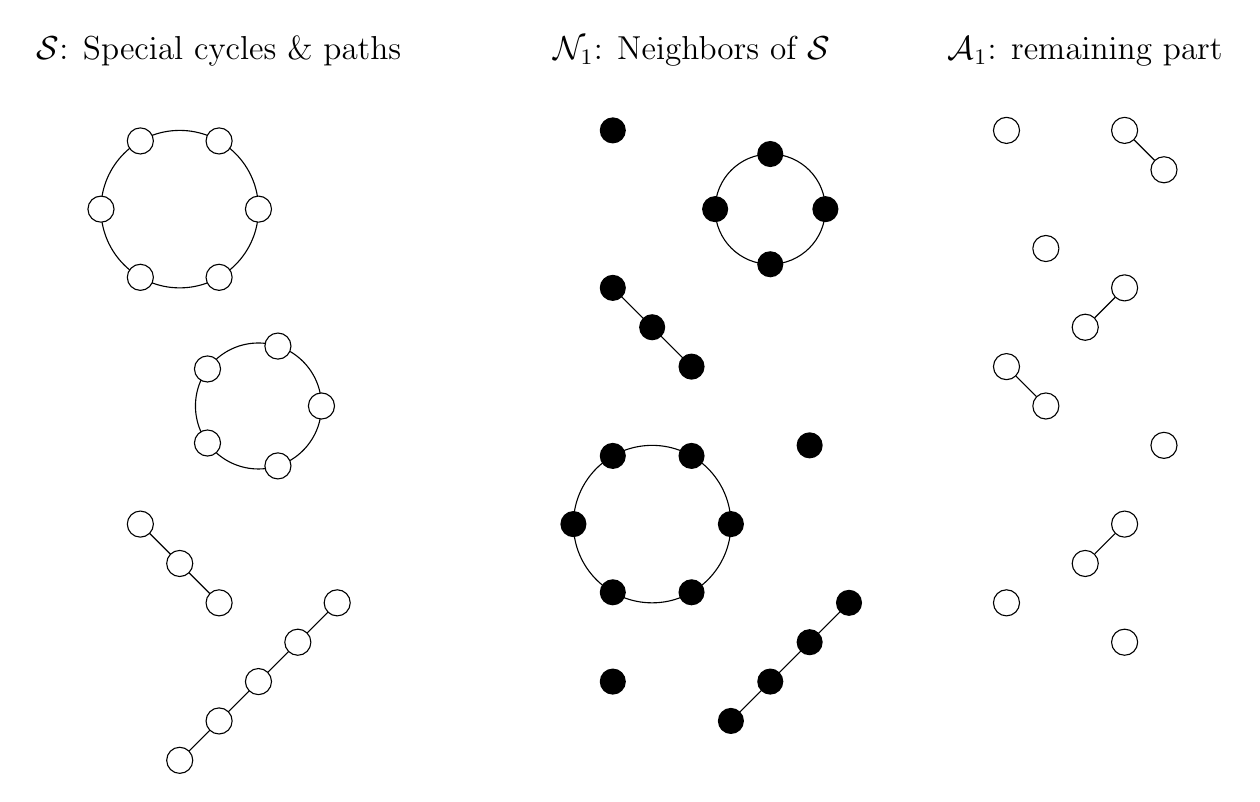
\begin{tikzpicture}
[node distance=1cm,
V/.style={draw,circle,fill=white},
N/.style={circle,fill=black},
dedge/.style={black,>=latex', shorten >=.0pt, shorten <=.0pt},
myedge/.style={thick}]
%%
%%%%%%%%%%%%%%%%%%
% S
%%%%%%%%%%%%%%%%%%
\node at (0,5) {\large{$\mS$: Special cycles \& paths}};
%% cycle 1
\begin{scope}[xshift=-.5cm,yshift=3cm]
\def \n {6}
\def \rad {1cm}
\node[V] at ({360/\n * 0}:\rad) {};
\node[V] at ({360/\n * 1}:\rad) {};
\node[V] at ({360/\n * 2}:\rad) {};
\node[V] at ({360/\n * 3}:\rad) {};
\node[V] at ({360/\n * 4}:\rad) {};
\node[V] at ({360/\n * 5}:\rad) {};
%%
\begin{pgfonlayer}{background}
\draw (0,0) circle(\rad);
\end{pgfonlayer}
%%
\end{scope}
%% cycle 2
\begin{scope}[xshift=0.5cm,yshift=0.5cm]
\def \n {5}
\def \rad {.8cm}
\node[V] at ({360/\n * 0}:\rad) {};
\node[V] at ({360/\n * 1}:\rad) {};
\node[V] at ({360/\n * 2}:\rad) {};
\node[V] at ({360/\n * 3}:\rad) {};
\node[V] at ({360/\n * 4}:\rad) {};
%%
\begin{pgfonlayer}{background}
\draw (0,0) circle(\rad);
\end{pgfonlayer}
%%
\end{scope}
%% path 1
\begin{scope}[xshift=0cm,yshift=-2cm]
\node[V] at (0,0) {};
\node[V] at (-.5,.5) {};
\node[V] at (-1,1) {};
%%
\begin{pgfonlayer}{background}
\draw (0,0) -- (-1,1);
\end{pgfonlayer}
\end{scope}
%%
%% path 2
\begin{scope}[xshift=-.5cm,yshift=-4cm]
\node[V] at (0,0) {};
\node[V] at (.5,.5) {};
\node[V] at (1,1) {};
\node[V] at (1.5,1.5) {};
\node[V] at (2,2) {};
%%
\begin{pgfonlayer}{background}
\draw (0,0) -- (2,2);
\end{pgfonlayer}
\end{scope}
%%
%%%%%%%%%%%%%%%%%%
% N1
%%%%%%%%%%%%%%%%%%
\begin{scope}[xshift=6cm,yshift=0cm]
\node at (0,5) {\large{$\mN_1$: Neighbors of $\mS$}};
%% cycle 1
\begin{scope}[xshift=-.5cm,yshift=-1cm]
\def \n {6}
\def \rad {1cm}
\node[N] at ({360/\n * 0}:\rad) {};
\node[N] at ({360/\n * 1}:\rad) {};
\node[N] at ({360/\n * 2}:\rad) {};
\node[N] at ({360/\n * 3}:\rad) {};
\node[N] at ({360/\n * 4}:\rad) {};
\node[N] at ({360/\n * 5}:\rad) {};
%%
\begin{pgfonlayer}{background}
\draw (0,0) circle(\rad);
\end{pgfonlayer}
%%
\end{scope}
%% cycle 2
\begin{scope}[xshift=1cm,yshift=3cm]
\def \n {4}
\def \rad {.7cm}
\node[N] at ({360/\n * 0}:\rad) {};
\node[N] at ({360/\n * 1}:\rad) {};
\node[N] at ({360/\n * 2}:\rad) {};
\node[N] at ({360/\n * 3}:\rad) {};
%%
\begin{pgfonlayer}{background}
\draw (0,0) circle(\rad);
\end{pgfonlayer}
%%
\end{scope}
%%
%% path 1
\begin{scope}[xshift=0cm,yshift=1cm]
\node[N] at (0,0) {};
\node[N] at (-.5,.5) {};
\node[N] at (-1,1) {};
\begin{pgfonlayer}{background}
\draw (0,0) -- (-1,1);
\end{pgfonlayer}
\end{scope}
%%
%% path 2
\begin{scope}[xshift=0.5cm,yshift=-3.5cm]
\node[N] at (0,0) {};
\node[N] at (.5,.5) {};
\node[N] at (1,1) {};
\node[N] at (1.5,1.5) {};
\begin{pgfonlayer}{background}
\draw (0,0) -- (1.5,1.5);
\end{pgfonlayer}
\end{scope}
%%
%% vertices
\node[N] at (-1,4) {};
\node[N] at (1.5,0) {};
\node[N] at (-1,-3) {};
%%
\end{scope}
%%%%%%%%%%%%%%%%%%
% A
%%%%%%%%%%%%%%%%%%
%% path 1
\begin{scope}[xshift=11cm,yshift=-1.5cm]
\node at (0,6.5) {\large{$\mA_1$: remaining part}};
%% edges 
\node[V] (a) at (0,0) {};
\node[V] (b) at ($(a)+(.5,.5)$) {};
\draw (a) -- (b);
%%
\node[V] (a) at (0,3) {};
\node[V] (b) at ($(a)+(.5,.5)$) {};
\draw (a) -- (b);
%%
\node[V] (a) at (-.5,2) {};
\node[V] (b) at ($(a)+(-.5,.5)$) {};
\draw (a) -- (b);
%%
\node[V] (a) at (1,5) {};
\node[V] (b) at ($(a)+(-.5,.5)$) {};
\draw (a) -- (b);
%%
%% vertices
\node[V] at (-1,5.5) {};
\node[V] at (-.5,4) {};
\node[V] at (0.5,-1) {};
\node[V] at (-1,-.5) {};
\node[V] at (1,1.5) {};
%%
\end{scope}
%%
\end{tikzpicture}
{}
\end{document}
